\documentclass[12pt]{article}


\usepackage{fullpage,enumitem,amsmath,amsfonts,amssymb,amsthm,graphicx}
\usepackage{array} % Improves `tabular` and `array` environments
\usepackage{pict2e} % Allows \linethickness{...} in diagonal lines
\usepackage{diagbox}


\newcommand{\Z}{\mathbb{Z}}
\newcommand{\R}{\mathbb{R}}
\newcommand{\C}{\mathbb{C}}
\newcommand{\Q}{\mathbb{Q}}
\newcommand{\N}{\mathbb{N}}
\newcommand{\F}{\mathbb{F}}
\newcommand{\E}{\mathbb{E}}
\newcommand{\Exp}[1]{\text{exp}(#1)}
\newcommand{\Diag}[1]{\text{Diag}(#1)}
\newcommand{\norm}[1]{\left\Vert #1\right\Vert}
\newcommand{\Span}[1]{\text{Span}(#1)}
\newcommand{\Cov}[1]{\text{Cov}(#1)}

\newenvironment{solution}{\vspace{0.2cm} \textbf{Solution.}}{}
\setlength{\parindent}{0pt}

% ------------------------------------------------------------------- %

\title{\vspace{-3cm}2801.001 Spring 2018 Homework 1 }
\author{Martin Arienmughare -- \texttt{moa258}\\
		Madhur Bhattad-- \texttt{mb6854}\\
		Louis Guigo -- \texttt{lg2894}\\
		Mario Zhu -- \texttt{mz833}}
\date{April 2018}

% ------------------------------------------------------------------- %

\begin{document}
	\maketitle
\textbf{Submission instructions:} Groups of three to four, due 14 calendar days after the homework is posted, in
electronic format. Submission must contain: (a) master answer sheet (typewritten or handwritten) with
header containing your names and NetIDs, and (b) all relevant computer files such as code source, Excel
files etc.

	\noindent
	\rule{\linewidth}{0.4pt}
	
	\section*{Problem 1}
You are short 100 at-the-money call option contracts on the S\&P 500 index expiring in one year with a contract multiplier of 100. The current index level is 2600, the interest and dividend rates are zero.

	\begin{enumerate}[label=(\alph*)]
		\item Simulate the evolution of the index level at periods Δt as a geometric Brownian motion with volatility $\sigma$ (free parameter) and calculate the corresponding call value, delta, gamma and theta using a fixed 20\% implied volatility.
		
		\begin{solution}
		
		[TODO]
	
		\end{solution}
		\item Then simulate your actual cumulative P\&L when periodically delta-hedging your position (assuming you can trade the index as an asset) and compare it against the proxy formula on slide 11 for the following matrix of parameters:
		
		\linethickness{1pt}
		\setlength{\arrayrulewidth}{1pt}
		\begin{tabular}{|c|c|c|c|}
			\hline
			\backslashbox{$\sigma$}{$\Delta t$} & Monthly (12 per year) & Weekly (52 per year) & Daily (252 per year) \\ \hline
			$\sigma = 25 \%$ &  &  &  \\ \hline
			$\sigma = 20 \%$ &  &  &  \\ \hline
			$\sigma = 15 \%$ &  &  &  \\ \hline
		\end{tabular} 
	
		\begin{solution}
		
		[TODO]
		
		\end{solution}
		
		\item Provide a statistical analysis of your results over 10,000 simulations, where one simulation is an entire index path.
		
		\begin{solution}
		
		[TODO]
			
		\end{solution}
	\end{enumerate}
	
\newpage

	\section*{Problem 2}
Use your knowledge of how the VIX is calculated to show that the VIX is not the price of an investable asset. What about the square of the VIX?

\begin{solution}

VIX is calculated from the fair short term variance of listed options on S\&P 500. The fair short term variance is in accordance with the fair strike of a variance swap calculated using price of a log contract with payoff as $-\log (\frac{S(T)}{F})$, where F is the price of forward of the underlying S with corresponding maturity. 

Since VIX is just an index, the only possible way to invest in VIX is by replicating the index. Unlike other indexes like S\&P 500, replicating VIX using S\&P 500 options seems complicated as the time value factor associated with VIX is just the square root of the time value factor that is associated with risk neutral discounting. (Since the formula for VIX calculation, has the risk neutral time value factor $e^{rT}$ associated with the squared of the VIX)

Therefore the only way to invest in VIX is via VIX futures and VIX options.

VIX squared on the other hand, as described by the calculation of fair short term variance, is just $\frac{2}{T}$ times the risk neutral expectation of the log contract. Thus the VIX squared can be invested using variance swaps.

Hence while VIX is not the price of an investable asset, VIX squared is. 

\end{solution}

\newpage
	
	\section*{Problem 3}
On March 29, 2018 the S\&P 500 index (SPX) is 2611.53 and the 12-month VIX is 21.28. The implied volatility smile of SPX options expiring on March 15, 2019 is given as:
$$ \sigma^* = \sqrt{a + b \left( \rho (x - m)  + \sqrt{(x-m)^2 + s^2} \right)} $$
where $a = 0.009$, $b = 0.11$, $\rho = −0.12$, $m = 0.2$, $s = 0.05$, $x = \log \frac{K}{F}$ is log-moneyness and $F = 2625.10$ is the forward price. The continuous interest rate is 2.09\% p.a.

	\begin{enumerate}[label=(\alph*)]
	\item Draw the implied volatility smile curve for strikes $500 \leq K \leq 5000$.
	
	\begin{solution}
	
	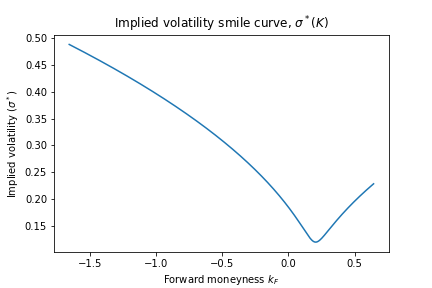
\includegraphics{impliedVol.png}
	
	\end{solution}
	
	\item Calculate the fair strike K var of a variance swap expiring on March 15, 2019 with the method of your choice. How close is your calculation to the 12-month VIX? Why is it not exactly the same?
	
	\begin{solution}
	
	Applying $Eq. (5.3)$ from the Advanced Equity Derivatives text to options data obtained from the CBOE on April 18 (3:28PM), resulted in the fair strike, $K_{var}=19.0.$  The strikes of the puts (calls) used were at most (least) the forward price.
	The results obtained are quite close the the 12-month VIX, with a percentage error of $11.8\%.$  They are not exactly the same because variance is convex in volatility, and the difference between them is related to the volatility of the volatility.
	
	
	\end{solution}	

	\end{enumerate}

\newpage

	\section*{Problem 4}
Consider a real symmetric matrix $A$. Show that $\Exp{A} = \sum_{n=0}^{\infty} \frac{A^n}{n!}$ is symmetric positive-definite.
Hint: Use spectral decomposition.

	\begin{solution}
		
	Let $A \in S_n(\R)$. Let us prove that $\Exp{A} \in S_n^{++}(\R)$.
	\begin{enumerate}[label={\arabic*.}]
		\item The linear application $M \mapsto M^T$ is continuous on $\mathcal{M}_n(\R)$, so if $A$ is symmetric, we have $\Exp{A}^T = \Exp{A}$; $\Exp{A}$ is symmetric.
		\item Since $A$ is symmetric, there exists an orthonormal basis of diagonalization of A, i.e.\:
		$$ A = P \Diag{\lambda_1, \ldots, \lambda_n} P^{-1}$$
		with $P \in O_n(\R)$ and $\lambda_1,\ldots,\lambda_n \in \R$.
		Taking the exponential of A, we therefore have:
		$$ \Exp{A} = P \Diag{e^{\lambda_1}, \ldots, e^{\lambda_n}} P^{-1}$$
		With this writing, we clearly see that all the eigenvalues of $\Exp{A}$ are strictly positive. Therefore $\Exp{A}$ is positive-definite.
	\end{enumerate}
	
	With these two points, $\Exp{A}$ is a symmetric positive-definite matrix: $\Exp{A} \in S_n^{++}(\R)$.
	\end{solution}
	
\newpage

	\section*{Problem 5}

Let $(\Omega, \mathcal{A}, \mathbb{P})$ be a probability space, and $E$ the vector space of random variables with finite second moment and mean zero. Define $\langle X, Y \rangle = \Cov{X, Y}$ and, for any event $A \in \mathcal{A}$, $Z_A = I_A - \mathbb{P}(A)$ where $I_A$ is the indicator variable of $A$.

	\begin{enumerate}[label=(\alph*)]
		\item Show that $\langle \cdot,\cdot \rangle$ is an inner product on $E$. What is the induced norm?
		
		\begin{solution}		
			
		Let us recall that, for $X$ and $Y$ random variables, we define the covariance by:
		
		$$ \Cov{X,Y} = \E ((X - \E(X)) (Y -\E(Y)))$$
		
		Relation from which we deduce by some algebra:
		$$\Cov{X,Y} = \E(XY) - \E(X)\E(Y)$$
		
		Over $E$, it simplifies to $\Cov{X,Y} = \E(XY)$
		
		Let us check that $X,Y \mapsto \langle X,Y \rangle$ is an inner product on $E$, the vector space of real random variables with zero mean and finite second moment.
		
		$\Cov{\cdot,\cdot}$ is an application from $E \times E$ to $\R$.
		
		Let $X,Y,Z \in \E$ and $\lambda \in \R$.
		\begin{enumerate}[label={\roman*)}]
			\item \textit{(Symmetry)} $\Cov{X,Y} = \Cov{Y,X}$, clearly, using the symmetry in $X,Y$ in the definition of the covariance.
			\item \textit{(Linearity)} $\Cov{\lambda X, Y} = \E ((\lambda X - \E(\lambda X)) (Y -\E(Y))) = \lambda \E ((X - \E(X)) (Y -\E(Y))) = \lambda \Cov{X,Y}$, by linearity of the expectation.
			
			Besides: $\Cov{X +Z, Y} =  \E ((X + Z - \E(X +Z)) (Y -\E(Y))) = \E ((X - \E(X) + Z - \E(Z)) (Y -\E(Y))) =  \E ((X - \E(X))(Y-\E(Y))) +  \E ((X - \E(X))(Y-\E(Y))) = \Cov{X,Y} + \Cov{Z,Y}$. 
			
			\item \textit{(Positive)}  $\Cov{X,X} = \E ((X - \E(X))^2) \geqslant 0$ by positivity of the random variable $(X-\E(X))^2$ and monotony of the expectation.
			\item \textit{(Definite)} $\Cov{X,X} = 0$ \textit{iff} $(X-\E(X))^2 = 0$ since it is a positive random variable. This implies that$X-\E(X)=0$ , i.e.\ $X=0$ since $\E(X) = 0$ by definition of $E$. 
		\end{enumerate}
	
		With these elements, $\Cov{\cdot,\cdot}$ is an inner product on $E$. The induced norm is:
		
		$$ \norm{X} = \sqrt{\E(X^2)} $$
			
		\end{solution}
		\item Show that $|\rho(X, Y)| \leq 1$ (correlation coefficient).
	
		\begin{solution}
			
		By definition, $\rho(X, Y) = \frac{\langle X,Y \rangle}{\norm{X}\norm{Y}}$. But $\langle X,Y \rangle \leq \norm{X}\norm{Y}$ by Cauchy-Schwarz inegality, so $\rho \leq 1$.
			
		\end{solution}
		\item Show that if $X, Y \in E \setminus \{0\}$ are probabilistically independent then $X, Y$ are linearly independent within $E$. Converse?
		
		\begin{solution}
			
		Let us reason by contraposition.
		Let us assume that $X,Y$ are not linearly independent, i.e.\ there exists $\lambda \in \R$ such that $Y = \lambda X$. Necessarily, $\lambda \neq 0$ since $X,Y \neq 0$.
		
		So for $x,y \in \R$, $\mathbb{P}(X=x, Y=y) = \mathbb{P}(X=x, X= \frac{y}{\lambda})$.
		Therefore, $\mathbb{P}(X=x, Y=y) = 0$ if $y \neq \frac{x}{\lambda}$ and $\mathbb{P}(X=x)$ else.
		In that second case, we see that $\mathbb{P}(X=x, Y=y) \neq \mathbb{P}(X=x) \mathbb{P}(Y=y) = \mathbb{P}(X=x)^2$, unless $X$ is constant equal to $x$ which is impossible by assumption since $X \neq 0$ and $\E(X) = 0$ by definition of the vector space $E$.
		
		Therefore, $X$ and $Y$ are not probabilistically independent.
		
		This proves the direct implication over $E$.
		
		The converse is false. As a counterexample, consider the random variable $X$ taking values in the set $\{-1,0,1\}$ with equal probabilities $\frac{1}{3}$, and take $Y = X^2$.
		
		Clearly, $X$ and $Y$ are linearly independent (since the probability affected to the outcome $-1$ is non zero in the law of $X$).
		However, $X$ and $Y$ are probabilistically dependent since for instance $\mathbb{P}(X = 0, Y = 1) = 0 \neq \mathbb{P}(X=0)\cdot \mathbb{P}(Y=1) = \frac{1}{3} \cdot \frac{2}{3}$.
		
		\end{solution}
		\item Let $X, Y \in E \setminus \{0\}$ . What is the statistical interpretation of the orthogonal projection of $Y$ on $\Span	{X}$?
		
		\begin{solution}
		
		The orthogonal projection of $Y$ on the line $\Span	{X}$ is exactly given by: $$ \Pi_{\Span	{X}}(Y)= \frac{\langle X, Y \rangle}{\norm{X}}X = \frac{\Cov{X,Y}}{Var(X)}X$$
		This orthogonal projection is a random variable linearly dependent with $X$, which has the same correlation with $X$ as $Y$ has. Additionally, $\frac{\Cov{X,Y}}{Var(X)}$ is the $\lambda$ coefficient that minimizes the variance of any random variable $Y - \lambda X$.
		
		In statistical terms, it means that if we wanted to predict $Y$ using $X$ with a linear model, i.e.\ $\hat{Y} = \alpha X + \beta$, $\frac{\Cov{X,Y}}{Var(X)}$ would be the $\alpha$ coefficient that minimizes the norm of the prediction error $\epsilon = \E((\hat{Y} - Y)^2)$.
		
		Indeed the first order conditions of this simple minimization problem are:
		
		$$\frac{\partial \epsilon}{\partial \alpha} = - 2 \E ((\hat{Y}-Y)\frac{\partial \hat{Y}}{\partial \alpha}) \text{ and } \frac{\partial \epsilon}{\partial \beta} = - 2 \E ((\hat{Y}-Y)\frac{\partial \hat{Y}}{\partial \beta})$$
		which can be rewritten:
		$$\E((\hat{Y}-Y)X) = 0 \text{ and } \E(\hat{Y} - Y) = 0$$
		
		This means that the prediction error $\hat{Y} - Y$ has to be orthogonal to X and that its expected value must be zero. Note that the first order conditions correspond to a minimum given the positive-definiteness of the Hessian.
		
		Substituting $\hat{Y} = \alpha X + \beta$, we obtain $\alpha = \frac{\Cov{X,Y}}{Var(X)}$ and $\beta = \E(Y) - \frac{\Cov{X,Y}}{Var(X)} \E(X)$. As stated above, it means that $\frac{\Cov{X,Y}}{Var(X)} X$ is the closest random variable (i.e.\ the one that minimizes the variance of the prediction error) to $Y$ in $\Span{X}$.

		Besides, the prediction error is given by $\epsilon = (1 - \rho^2)Var(Y)$. If $\rho = \pm 1$, a perfect prediction can be made.
		When $\rho = 0$, the variance in the prediction is as large as the variation in Y, which implies that the predictor is very bad.
		For intermediate values of $\rho$, the predictor reduces the error.
		
		\end{solution}
		\item Verify that $Z_A \in E$ and calculate $\langle Z_A , Z_B \rangle$ for any $A,B \in \mathcal{A}$. When is $Z_A \perp Z_B$ ? Are $Z_A, Z_{\overline{A}} $ linearly independent in E?
		
		\begin{solution}
		
		It is a fact that $Z_A \in E$ for any $A\in \mathcal{A}$ since this is a random variable with first and second moment respectively such that: $\E(Z_A) = \E(I_A - \mathbb{P}(A)) = \E(I_A) - \mathbb{P}(A) = 0$ and $\E(Z_A^2) = \E(I_A^2 -2\mathbb{P}(A) I_A + \mathbb{P}(A)^2) = \E(I_A^2) -2\mathbb{P}(A)\E(I_A) + \mathbb{P}(A)^2 = \mathbb{P}(A) (1 - \mathbb{P}(A))$, so $\E(Z_A^2)\leq \infty$ since $I_A^2 = I_A$.
		
		Besides, for $A,B\in \mathcal{A}$, $\langle Z_A , Z_B \rangle = \langle I_A - \mathbb{P}(A) , I_B - \mathbb{P}(B) \rangle = \langle I_A, I_B \rangle - \langle I_A,\mathbb{P}(B) \rangle - \langle \mathbb{P}(A),I_B \rangle + \langle \mathbb{P}(A), \mathbb{P}(B) \rangle  = \langle I_A,I_B \rangle$
		
		So, $\langle Z_A , Z_B \rangle = \E((I_A - \mathbb{P}(A))(I_B - \mathbb{P}(B))) = \E(I_{A\cap B} - \mathbb{P}(B) I_A - \mathbb{P}(A) I_B + \mathbb{P}(A)\mathbb{P}(B))$.
		
		Id est, $\langle Z_A , Z_B \rangle= \mathbb{P}(A\cap B) - \mathbb{P}(A) \mathbb{P}(B)$.
		
		We can see that $Z_A \perp Z_B$ when $ \mathbb{P}(A\cap B) = \mathbb{P}(A) \mathbb{P}(B)$, that is, when events $A$ and $B$ are stochastically independent.
		
		
		$Z_A, Z_{\overline{A}} $ are not linearly independent in $E$ since for any $Z_{\overline{A}} = 1 - Z_A$.
		\end{solution}
		\item Suppose $A, B \in \mathcal{A} \setminus \{\emptyset, \Omega\}$ are disjoint, and $B \neq \overline{A}$. Show that $Z_A, Z_B$ are linearly independent.
		
		\begin{solution}
			
		Let $A, B \in \mathcal{A} \setminus \{\emptyset, \Omega\}$ such that $A\cap B = \emptyset$.
				Let $\lambda, \mu \in \R$ such that $\lambda Z_A + \mu Z_B = 0$.
		
		Since $A\cap B = \emptyset$, plugging in any two elementary events $x\in A$ and $y \in B$ yields:
		
		\[
		\begin{cases}
			-\lambda \mathbb{P}(A) + \mu (1 - \mathbb{P}(B) = 0 \\ \lambda (1 - \mathbb{P}(A)) - \mu \mathbb{P}(B) = 0
		\end{cases} 
		\]
		
		Taking the difference between these equations, we obtain the condition: $\lambda = \mu$.
		
		Therefore, $\lambda (Z_A + Z_B) =0$. Since $B \neq \overline{A}$, this implies $\lambda = \mu = 0$.
		
		Thus, $Z_A$ and $Z_B$ are linearly independent.
		
		\end{solution}
		\item Suppose $A \in \mathcal{A} \setminus \{\emptyset, \Omega\}$ and define $B = \{\emptyset, A, \overline{A}, \Omega\} \subseteq A$. Let $Y = E(X|B)$. Verify that $Y \in E$ and show that $Y$ is the orthogonal projection of $X$ on $\Span{Z_A}$.
			 
		\begin{solution}
		
		Note that $B$ is a $\sigma$-Algebra, therefore it makes sense to consider $Y=\E(X|B)$.
		
		Let us recall that $Y$ is defined as the almost surely unique random variable such that for any bounded and $B$-measurable random variable $U$, $\E(XU) = \E(YU)$. 
		
		We have: $\E(Y) = \E(\E(X|B)) = \E(X) = 0$ using the tower property of conditional expectation and the fact that $X \in E$.
		
		Besides, $\E(Y^2) = \E(\E(X|B)^2) \leq \E(\E(X|\sigma(X))^2$ $\leq \E(X^2) \leq \infty$ since $X \in E$.
		
		Let us check that $Y$ is the orthogonal projection of $X$ on $\Span{Z_A}$. For that matter, let us show that it is such that for all $U \in \Span{Z_A}$, $\langle X- Y, U \rangle = 0$.
		
		Let $U \in \Span{Z_A}$. Since $Z_A$ is $B$-measurable, $U$ is also $B$-measurable, and it follows that $\E(UX|B) = U \E(X|B)$.
		
		Therefore: $\E(U \E(X|B)) = \E(\E(UX|B)) = \E(UX)$ i.e.\ $\langle U, Y \rangle = \langle U, X \rangle$. That is exactly $\langle U, Y - X \rangle = 0$.
		
		Since this is true for any $U \in \Span{Z_A}$, we conclude that $Y - X = \E(X|B) - X$ realizes the minimum distance from $X$ to $\Span{Z_A}$.
		
		Since $(E, \Cov{\cdot,\cdot})$ is a Hilbert space, the minimum distance is realized by the orthogonal projection. Thus, we have $Y = \Pi_{\Span{Z_A}}(X)$.
		
		\end{solution}
	\end{enumerate}

\newpage

	\section*{Problem 6}
	Consider a vector space $E$ equipped with a norm $N(x)$.

	\begin{enumerate}[label=(\alph*)]
		\item Show that $N$ is Euclidean (i.e.\ induced by some inner product) if and only if $N$ satisfies the parallelogram law: $$N(x + y)^2 + N(x - y)^2 = 2 \cdot [N(x)^2 + N(y)^2]$$
		Hint: Define the inner product through $N$.
	
		\begin{solution}
		
		If $N$ is Euclidean, it derives from a certain inner product $\langle \cdot,\cdot \rangle$. And we have:
		$$ N(x+y)^2 + N(x-y)^2 = \langle x+y,x+y \rangle + \langle x-y,x-y \rangle = 2 \langle x,x\rangle  + 2 \langle y,y \rangle + 2\langle x,y\rangle -2\langle x,y\rangle$$
		$$ \text{Therefore, }N(x+y)^2 + N(x-y)^2 = 2 \cdot \left[ N(x)^2 + N(y)^2 \right]$$
		
		Let's now assume that $N$ checks the parallelogram law, and let us prove that the bilinear form $\langle \cdot,\cdot \rangle$ defined by polarization as follows is an inner product over $E$ from which $N$ derives:
		$$ \langle x,y\rangle = \frac{1}{4} \cdot \left[ N(x+y)^2 - N(x-y)^2 \right]$$
		
		We clearly have, by homogeneity, $N(x) = \sqrt{\langle x,x \rangle}$.
		
		$\langle \cdot,\cdot \rangle$ is an application from $E \times E$ to $\R$.
		
		Let $x,y,z \in \E$ and $\lambda \in \R$.
		\begin{enumerate}[label={\roman*)}]
			\item \textit{(Symmetry)} $\langle x,y\rangle = \langle y,x\rangle$, clearly, using the symmetry in $x,y$ in its definition.
			\item \textit{(Positive)}  $\langle x,x \rangle = \frac{1}{4} \cdot N(2x)^2 = N(x)^2 \geqslant 0$ since $N(0) = 0$ by separation.
			\item \textit{(Definite)} $\langle x,x \rangle = 0$ \textit{iff} $\frac{1}{4}N(x)^2 = 0$ \textit{iff} $x=0$ by separation.
			\item \textit{(Linearity)} Observe that: $$\langle x+y, z \rangle + \langle x-y,z \rangle = \frac{1}{4} \left[ N(x+y+z)^2 - N(x+y-z)^2 + N(x-y+z)^2 - N(x-y-z)^2 \right]$$
			Therefore,
			$$\langle x+y, z \rangle + \langle x-y,z \rangle = \frac{1}{4} \left[ 2\cdot \left[ N(x+y)^2 - N(z)^2 \right] + 2 \cdot \left[ N(x-y)^2 + N(z)^2 \right] \right]$$
			Thus,
			$$ \langle x+y, z \rangle + \langle x-y,z \rangle = 2 \cdot \left[ N(x)^2 + N(y)^2\right]$$
			Which can be rewritten:
			$$ \langle x+y, z \rangle + \langle x-y,z \rangle = 2 \cdot \langle x,y \rangle$$
			From which we deduce, taking $y=x$:
			$$ \langle 2 \cdot x, y \rangle = 2 \cdot \langle x,y \rangle$$ 
			
			By induction, we prove that this it is true for any power $n$ that:
			$$ \langle 2^n \cdot x, y \rangle = 2^n \cdot \langle x,y \rangle $$
			
			Taking $u = \frac{1}{2}(x+y)$ and $v = \frac{1}{2} (x-y)$, we have:
			$$ \langle x+y,z  \rangle = \langle 2 \cdot u,z \rangle = 2 \cdot \langle u, z\rangle = \langle u +v, z \rangle + \langle u-v, z \rangle = \langle x, z\rangle + \langle y,z \rangle$$.
			
			By induction we conclude that for any $n \in \N$ (we've seen that it's true for $n=0$), and any $x,y \in E$ we must have:
			$$\langle nx,y \rangle = n \langle x,y \rangle$$
			
			We can extend the linearity to $\Z$ using $\langle -x,y\rangle = - \langle x, y \rangle$, and then to $\Q$ using $\langle x,y \rangle = n \cdot \langle \frac{1}{n} x,y \rangle$.
			
			We conclude that the linearity is true over $\R$ using the well-known density of $\Q$ in $\R$ and the continuity of the application $(x,y) \mapsto \frac{1}{4} \cdot \left[ N(x+y)^2 - N(x-y)^2 \right]$, since the norm $N$ is continuous.
			
			Therefore, the linearity of $\langle \cdot, \cdot \rangle$ is true.
			
			Therefore $\langle \cdot, \cdot \rangle$ is an inner product over $E$ from which $N$ derives since $N(x) = \sqrt{\langle x,x \rangle}$.
			
			\underline{Conclusion:} $N$ is a Euclidean norm if and only if it checks the parallelogram identity.
			
		\end{enumerate}
		
		\end{solution}
		\item Which of the following are Euclidean norms on $E = R^n$?
		$$N_p (x) = \sqrt[p]{\sum_{i=1}^{n} |x_i|^p}$$
		$$Q_p (x) = \sqrt{N_2 (x)^2 + \frac{1}{p} \sum_{i < j} x_i x_j} $$
		where $p \in [1, \infty)$.
		
		\begin{solution}
		
		Given the previous question, we just need to verify if these norms check the parallelogram identity to know if they are Euclidean.
		
		For $p = 2$, $N_p$ is nothing but the so called Euclidean norm over $\R^n$, which as its name tells us, is Euclidean and derives from the canonical inner product of $\R^n$: $\langle x,y \rangle = x^T y$.
		
		However, \textbf{for} $p \geq 1$ \textbf{but} $p\neq 2$, $N_p$ is not Euclidean.
		As a counterexample, one can consider $x = (1,1,0, \ldots, 0)$ and $y = (1,-1,0,\ldots,0)$. We have $N_p(x) = N_p (y) = \sqrt[p]{2}$ but $N_p (x+y) = N_p (x-y) = 2$. So $N_p ^2 (x+y) + N_p ^2 (x-y) = 8 \neq 2 ( N_p ^2 (x) + N_p ^2 (y)) = 4 \sqrt[\frac{p}{2}]{2}$.
		
		Since it doesn't check the parallelogram identity, $N_p$ is not Euclidean \textbf{for} $p \geq 1$ \textbf{but} $p\neq 2$.
		
		$Q_p$ is not a norm for any $p \in [1, \infty)$ since it doesn't check the triangle inequality: for $x = (1,0,\ldots,0)$ and $y = (0,1,0,\ldots,0)$, we have:
		$$Q_p(x+y)^2 = 2^2 + \frac{1}{p} > Q_p(x)^2 + Q_p(y)^2 = 1^2 + 1^2 = 2$$
		
		A fortiori, it can't be a Euclidean norm.
		
		\end{solution}
		\item Define $A^2 (x, y) = [N(x) \cdot N(y)]^2 - [N(x + y)^2 - N(x - y)^2 ]^2 /16$. Show that if $N$ is Euclidean then
		$A^2 (x, y) \geq 0$ and $A(x + y, x - y)$ = $2 \cdot A(x, y)$.
		
		Geometric interpretation for $E = R^2$ ?
		
		\begin{solution}
		
		The triangle and reverse triangle inequalities tell us that for any $x,y \in E$:
		
		$$
		\left\{
		\begin{array}{ll}
		N(x+y) \leqslant N(x) + N(y)\\
		N(x-y) \geqslant | N(x) - N(y)|
		\end{array}
		\right.
		$$
		
		Since both sides are positive, we can compose by the square function and obtain:
		
		$$
		\left\{
		\begin{array}{ll}
		N(x+y)^2 \leqslant (N(x) + N(y))^2\\
		N(x-y)^2 \geqslant (N(x) - N(y))^2
		\end{array}
		\right.
		$$
		
		Taking the negative version of the second inequality and adding them, we get:
		
		$$
		N(x+y)^2 - N(x-y)^2 \leqslant (N(x) + N(y))^2 - (N(x) - N(y))^2
		$$
		
		After simplification, the right hand-side is exactly $4 N(x) N(y)$ so we get:
		
		$$
		\frac{1}{4} (N(x+y)^2 - N(x-y)^2) \leqslant N(x) N(y)
		$$
		
		To prove $A^2(x,y) \geqslant 0$, we need to show that $\frac{1}{16} (N(x+y)^2 - N(x-y)^2)^2 \leqslant (N(x) N(y))^2$, i.e.\ $\frac{1}{4} | N(x+y)^2 - N(x-y)^2 | \leqslant N(x) N(y)$.
		
		Given the first inequality proved, we just need to show that 
		
		$$- \frac{1}{4} (N(x+y)^2 - N(x-y)^2) \leqslant N(x) N(y)$$
		
		Given that $N$ is Euclidean, this is equivalent to:
		
		$$ 2 ( N(x)^2 + N(y)^2 - 2 N(x+y)^2) \leqslant 4 N(x) N(y)$$
		
		Itself equivalent to
		
		$$ N(x+y)^2 \geqslant (N(x) - N(y))^2$$
		
		Which is true by the second triangle inequality used above (it is its square).
		
		Conclusion:
		
		$$\frac{1}{4} | N(x+y)^2 - N(x-y)^2 | \leqslant N(x) N(y)$$
		
		i.e\
		
		$$\frac{1}{16} (N(x+y)^2 - N(x-y)^2)^2 \leqslant (N(x) N(y))^2$$
		
		i.e.\
		
		$$A^2(x,y) \geqslant 0$$
		
		Let us now prove that $A(x + y, x - y)$ = $2 \cdot A(x, y)$ (well defined with the first point).
		
		We have: $4 A^2(x,y)  = 4((N(x) N(y))^2 - \frac{1}{16} (N(x+y)^2 - N(x-y)^2)^2)$.
		
		Using the parallelogram identity, we substitute: $N^2(x), N^2(y), N^2(x+y), N^2(x-y) \leftarrow \frac{1}{2} (N^2(x+y) + N^2(x-y) - N^2(y)), \frac{1}{2} (N^2(x+y) + N^2(x-y) - N^2(x)), 2(N^2(x) + N^2(y)) - N^2(x-y), 2(N^2(x) + N^2(y)) - N^2(x+y)$.
		
		After draft calculations not reported here, we get exactly $$A^2(x + y, x - y) = 4 \cdot A^2(x, y) $$
		Taking the square root, $$A(x + y, x - y) = 2 \cdot A(x, y)$$

		In $\R^2$, $A^2$ represents the difference of squared surface between a rectangle with sides $N(x)$ and $N(y)$, and a rectangle with sides $\frac{N(x+y)}{2}$ and $\frac{N(x-y)}{2}$.
		
		So the last identity means that the difference of squared surface between a rectangle with sides $N(x+y)$ and $N(x-y)$, and a rectangle with sides $2N(x)$ and $2N(y)$ is equal to twice the difference of squared surface between a rectangle with sides $N(x)$ and $N(y)$, and a rectangle with sides $\frac{N(x+y)}{2}$ and $\frac{N(x-y)}{2}$.
		
		Quite unsatisfying interpretation...
		
		\end{solution}
	\end{enumerate}
	
\end{document}